\chapter{Критерии и показатели стойкости блочных симметричных шифров}

Основным и наиболее эффективным механизмом криптографической защиты информации
являются методы блочного симметричного криптографического преобразования.
Наряду с высокой скоростью преобразований и простотой практической реализации
симметричные криптоалгоритмы позволяют обеспечить высокую стойкость к различным
методам криптографического анализа.

Основным элементом современных блочных симметричных криптографических средств
защиты информации являются нелинейные узлы замен (нелинейные блоки подстановок),
качество построения которых непосредственновлияет на эффективность
разрабатываемых механизмов обеспечения безопасности информационных технологий.

На сегодняшний день в Украине нет национального алгоритма блочного симметричного
криптографического преобразования информации. Правила формирования нелинейных
узлов замен ныне действующего стандарта ГОСТ 28147-89 являются государственной
тайной Российской Федерации и не доступны для использования в Украине. В этом
смысле разработка математической модели и вычислительного метода формирования
нелинейных узлов замен с  высокими показателями стойкости является актуальной
научно-технической задачей, непосредственно связанной с выполнением ряда важных
государственных программ Украины и проводимым в недавнее время открытым
конкурсом симметричных криптографических алгоритмов.

Нелинейные узлы замен блочных  симметричных криптографических средств защиты
информации эффективно описываются в математическом виде совокупностью
криптографических булевых функций и накладываемой системой ограничений на
отдельные показатели стойкости. Таким образом, использование математического
аппарата булевой алгебры позволяет получить абстрактное аналитическое описание
нелинейных узлов замен и адекватно оценивать их стойкость.

В данном разделе исследуется структура и основные функциональные элементы
алгоритмов блочного симметричного криптографического преобразования информации,
обосновываются требования к перспективным методам блочного симметричного
криптографического преобразования, исследуется математический аппарат булевой
алгебры для построения нелинейных узлов замен  блочных симметричных
криптопреобразований, проводится анализ различных подходов к построению
нелинейных узлов замен, исследуются основные показатели стойкости нелинейных
узлов замен современных блочных симметричных шифров.

\section{Сравнительный анализ методов блочного симметричного криптографического
преобразования информации}

Для защиты информации с ограниченным доступом в современных информационных
системах применяются различные криптографические средства. Основным и наиболее
эффективным механизмом криптографической защиты информации являются методы
блочного симметричного криптографического преобразования. Наряду с высокой
скоростью преобразований и  простотой практической реализации симметричные
криптоалгоритмы позволяют обеспечить высокую стойкость к различным методам
криптографического анализа. Проведем анализ и сравнительное исследование методов
блочного симметричного  криптографического преобразования информации.

Как показывает анализ открытой литературы и результаты проводимых
криптографических конкурсов, на сегодняшний день реализовано большое число
различных блочных симметричных методов преобразования информации. При этом
подавляющее большинство методов делится на две большие группы: 

\begin{itemize}

    \item методы, построенные на основе использования цепей Фейстеля;

    \item методы, построенные на основе чередования процедур перестановок и
    подстановок, т.н. SP-конструкций. 

\end{itemize}

Приведём основные определения и обозначения блочных симметричных шифров и схем
их построения.

Пусть $T$ и $K$ "--- пространства текстов и ключей соответственно блочного
симметричного шифра.
\begin{equation}C = \{C_k: T \rightarrow T: k \in K\}\end{equation}

Пусть $r > 0$ "--- положительное целое и пусть $K_1, K_2, \ldots, K_r$ "--- $r$
конечных множеств. Говорят, что $C$ "--- $r$-раундовый итеративный блочный
симметричный шифр (БСШ), если он может быть записан в виде:
\begin{equation}C_k = R^{(r)}_{k_r} \circ R^{(r-1)}_{k_{r-1}} \circ \ldots \circ
R^{1}_{k_1}\end{equation}
для всех $k \in K$, где
\begin{equation}R^{(i)} = \{R^{(i)}_{k_i}: T \rightarrow T: k_i \in
K_i\}\end{equation}
называется $i$-м раундом $C$. 

Обычно $i$-й раунд блочного симметричного шифра состоит из трех слоев: слоя
подстановочного преобразования с использованием нелинейных блоков замен или
S-блоков,  слоя линейного перестановочного преобразования и  слоя функциональных
преобразований, таких как сдвиг, сложение по модулю с ключом и пр.

Такой итеративный подстановочно-перестановочный подход к разработке стойких
симметричных шифров был основан К. Шенноном и использует два общих принципа
построения: перемешивание (confusion) и рассеивание (diffusion). Перемешивание
осуществляет распространение влияния одного знака открытого текста на множество
символов шифртекста, что обуславливает лавинный эффект (в случае блочных шифров
"--- обеспечение распространения влияния каждого бита входного текста на все
биты выходного текста). Рассеиванием называется шифрующее преобразование,
нарушающее взаимосвязи статистических характеристик входного и выходного текста,
т.е. маскировку статистических свойств исходного сообщения.

Ключи $k_1, k_2, \ldots, k_r$ называются раундовыми ключами блочного
симметричного шифра и производятся из одного основного секретного ключа $k$
посредством детерминистического алгоритма, называемого алгоритмом распределения
ключей.

Схема Фейстеля (см. рис.~\ref{fig:feistel}) является структурой, которая
позволяет построить перестановку для $2n$-битных последовательностей,
основываясь на функциях от $n$-битных последовательностей. Обозначим схему
Фейстеля с $r > 0$ раундами преобразования, основанных на функциях $f_1, f_2,
\ldots, f_r: \{0, 1\}^n \rightarrow \{0, 1\}^n$ как $\Phi(f_1, f_2, \ldots,
f_r)$. Легко заметить, что $\Phi(f_1, f_2, \ldots, f_r)$ обратима, т.к.
\begin{equation}\Phi^{-1}(f_1, f_2, \ldots, f_r) = \Phi(f_r, f_{r-1}, \ldots,
f_1).\end{equation}

\begin{figure}
    \centering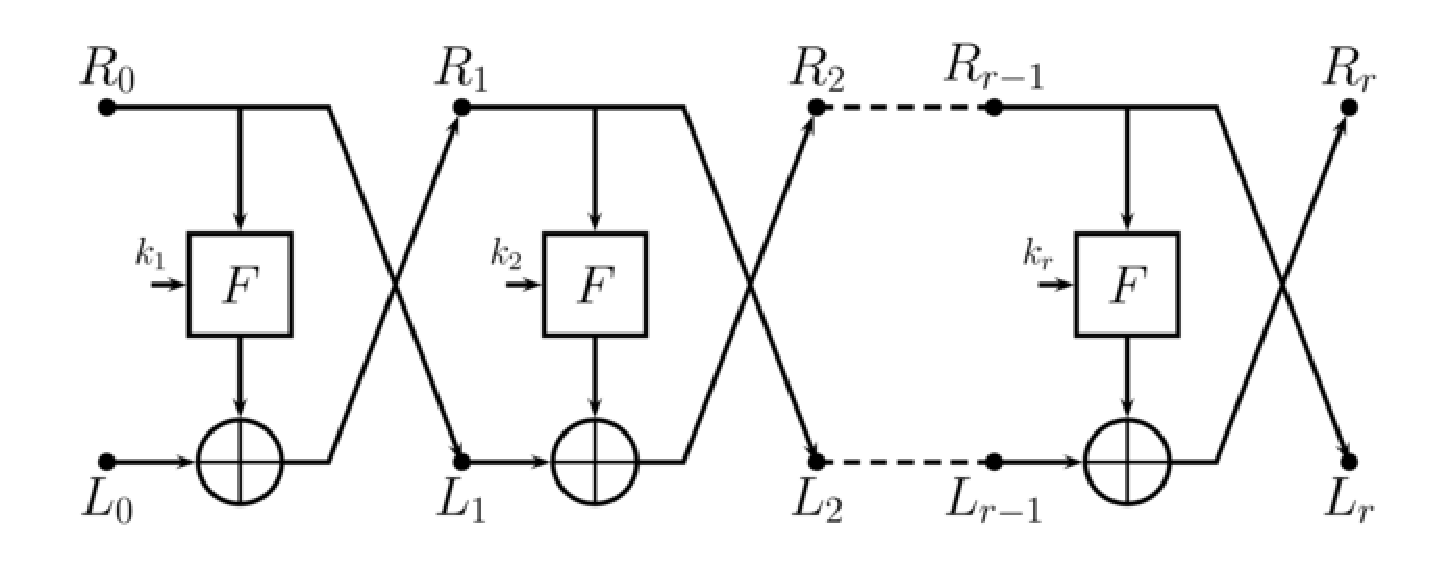
\includegraphics[width=1\textwidth]{feistel.eps}
    \caption{$r$–раундовая схема Фейстеля $\Phi(f_1, f_2, \ldots, f_r)$}
    \label{fig:feistel}
\end{figure}

Подстановочно-перестановочная структура (SP-структура, Substitution Permutation)
наиболее близка к принципам построения К. Шеннона и состоит из
последовательности слоев, в которых подстановочный слой осуществляет
перемешивание, за которым следует перестановочный слой, осуществляющий
рассеивание. SP-схема проиллюстрирована на рисунке~\ref{fig:SP}.

Все преобразования в SP-конструкциях должны быть обратимыми, так как
расшифрование производится путем выполнения обратных преобразований в обратном
порядке.

Оба вида  конструкций имеют свои достоинства и недостатки. Так, преимуществом
конструкции Фейстеля в сравнении с SP-конструкцией является значительное
облегчение практической реализации на процессорах малой разрядности, поскольку
обрабатываемые итеративной процедурой данные разбиваются на 2 блока и обработка
криптопримитивами производится над подблоками. Другим преимуществом является то,
что конструкция Фейстеля позволяет использовать в шифрующей функции более
широкий набор преобразований, так как к ним не предъявляется требование
обратимости.

\begin{figure}
    \centering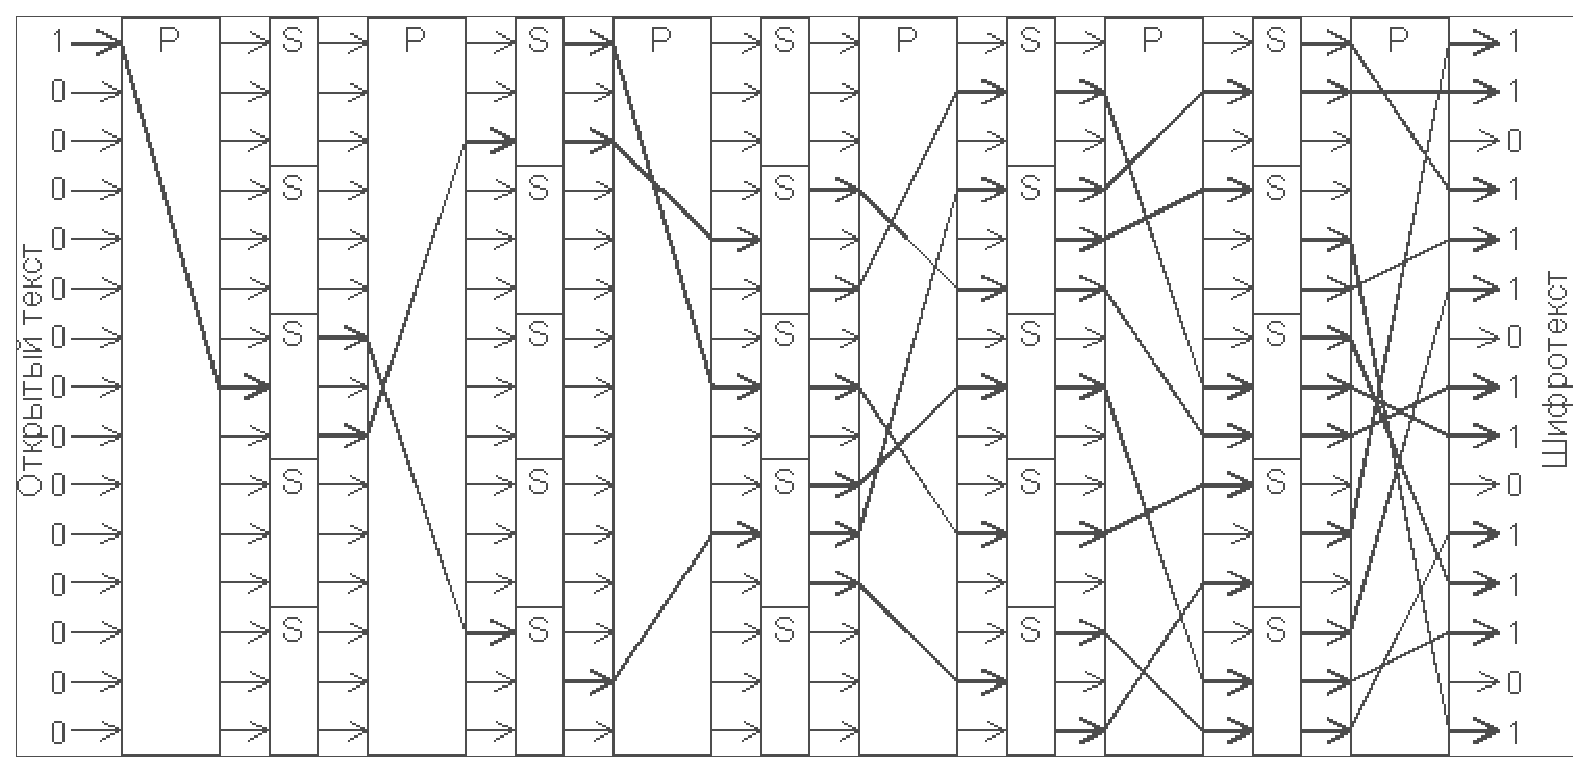
\includegraphics[width=1\textwidth]{sp.eps}
    \caption{SP-схема}
    \label{fig:SP}
\end{figure}

В то же время блоки подстановок и перестановок, применяемые в конструкциях
Фейстеля, имеют небольшой размер. Размерность же блоков нелинейного
подстановочного и линейного перестановочного преобразования в SP-конструкциях
значительно больше, что приводит к усилению устойчивости к различным методам
криптоанализа. Другим преимуществом SP структуры является ее большая
прозрачность и приближенность к принципам построения стойких симметричных шифров
К. Шеннона.

В соответствии с приведенными определениями и обозначениями, ниже приведены
результаты проведенного анализа современных БСШ (см.
табл.~\ref{table:BSC_parameters} - \ref{table:BSC_operations}). Рассматривались
БСШ, поданные на конкурс  NIST, на украинский конкурс, а также некоторые
распространенные конструкции. Отметим, что в таблице~\ref{table:BSC_parameters}
для шифров конкурса AES и украинского конкурса приводились данные только для
блоков длины 128 бит.

В 1997 г. NIST (National Institute of Standards and Technology, Национальный
Институт Стандартов и Технологий) объявил открытый конкурс на разработку
алгоритма блочного симметричного шифрования AES (Advanced Encryption Standard),
который должен был прийти на замену  DES (Data Encryption Standard) на несколько
следующих десятилетий. Пятнадцать алгоритмов шифрования, приведенных в
таблице~\ref{table:BSC_parameters}, были поданы в качестве кандидатов на конкурс
AES в 1998 г., затем пять алгоритмов были выбраны в качестве финалистов конкурса
в 1999 г.  Это MARS, RC6, Rijndael, Serpent и Twofish. Затем в 2001 г. в
качестве шифра AES был выбран блочный симметричный алгоритм Rijndael.

В 2006 г. в Украине был объявлен конкурс блочных симметричных шифров. Были
поданы пять алгоритмов шифрования: ADE, Лабиринт, Калина, Мухомор и RSB-32.
Из-за особенностей своей структуры шифр RSB-32 нельзя отнести к блочным
симметричным шифрам, поэтому он не приведен в
таблицах~\ref{table:BSC_parameters} - \ref{table:BSC_operations}.

Таблица~\ref{table:BSC_parameters} приводит общие параметры алгоритмов
рассматриваемых БСШ. Увеличение/уменьшение значений данных параметров влияет как
на стойкость блочных шифров, так и на скорость криптографического преобразования
информации.

{\def\arraystretch{1.15}
\begin{longtable}{| p{4cm} | C{3.5cm} | C{3.5cm} | C{4cm} |}
    \caption{\label{table:BSC_parameters}Параметры БСШ} \\ \hline
    Алгоритм    & Размер блока (в битах)    & Размер ключа (в битах)    & Число раундов     \\ \hline
    \endfirsthead
    \multicolumn{4}{r}{Продолжение таблицы \thetable} \\ \hline
    Алгоритм    & Размер блока (в битах)    & Размер ключа (в битах)    & Число раундов     \\ \hline
    \hline
    \endhead
    \hline
    \endlastfoot
    \multicolumn{4}{| c |}{Конкурс AES} \\ \hline
    CAST 256    & 128   & 128, 160, 192, 224, 256   & 48                        \\ \hline
    CRYPTON     & 128   & До 256                    & 12                        \\ \hline
    DEAL        & 128   & 128, 192.256              & 6, 8 (256-битный ключ)    \\ \hline
    DFC         & 128   & До 256                    & 8                         \\ \hline
    E2          & 128   & 128, 192, 256             & 12                        \\ \hline
    FROG        & 8-128 байт    & 5-125 байт        & 8                         \\ \hline
    HPC         & Любой размер  & 512               & 8                         \\ \hline
    LOKI97      & 128           & 128, 192, 256     & 16                        \\ \hline
    MAGENTA     & 128           & 128, 192, 256     & 6-8                       \\ \hline
    MARS        & 128           & 128-448           & 32                        \\ \hline
    RC6         & 128           & 128, 192, 256     & 20                        \\ \hline
    RIJNDAEL    & 128           & 128, 192, 256     & 10, 12, 14                \\ \hline
    SAFER+      & 128           & 128, 192, 256     & 8, 12, 16                 \\ \hline
    SERPENT     & 128           & 128, 192, 256     & 32                        \\ \hline
    TWOFISH     & 128           & 128, 192, 256     & 16                        \\ \hline

    \multicolumn{4}{| c |}{Распространённые шифры} \\ \hline
    DES         & 64            & 64 (56)           & 16                        \\ \hline
    BLOWFISH    & 64            & 32-448            & 16                        \\ \hline
    CAST 128    & 64            & 40-128            & 12, 16                    \\ \hline
    RC5         & 32, 64, 128   & 0-2040 (128)      & 0-255 (12)                \\ \hline
    SKIPJACK    & 64            & 80                & 32                        \\ \hline
    IDEA        & 64            & 128               & 8                         \\ \hline
    ГОСТ 28147-89  & 64            & 256               & 16, 32                    \\ \hline
    
    \multicolumn{4}{| c |}{Украинский конкурс} \\ \hline
    ADE         & 128           & 128, 192, 256     & 10, 12, 14                \\ \hline
    Лабиринт    & 128           & 128, 192, 256     & 8                         \\ \hline
    Калина      & 128           & 128, 256, 512     & 10, 14, 30                \\ \hline
    Мухомор     & 128           & 128, 256, 512     & 11                        \\ \hline
\end{longtable} }

Таблица~\ref{table:BSC_structures} классифицирует исследуемые
блочные симметричные шифры по их структуре. Таблица~\ref{table:BSC_operations}
приводит математические операции, на которых основаны рассматриваемые БСШ: ''XOR''
"--- исключающее побитовое ИЛИ w-битных слов, ''[+]'' "--- сложение по модулю 2
''$>>>$'' "--- циклический сдвиг вправо, ''$<<<$'' "--- циклический сдвиг влево.
''[-]'' "--- вычитание по модулю $2^w$, ''[$\cdot$]'' "---умножение по модулю
$2^w$.

Таблица~\ref{table:BSC_structures} показывает, что характерной особенностью
конструкций блочного криптографического преобразования информации является
использование в качестве шифрующих функций операций нелинейного перемешивания
(нелинейных S-блоков, или нелинейных узлов замен). Современные БСШ, не
использующие S-блоки, являются больше исключением из правил (RC6, RC5 и IDEA).

\begin{table}[ht]
    \def\arraystretch{1.15}
    \caption{Структуры БСШ}
    \label{table:BSC_structures}
    \begin{tabular}{| C{3.5cm} | C{4.5cm} | C{3.5cm} | C{3.5cm} |}
        \hline
        Схема Фейстеля  & Модифицированная схема Фейстеля   & SP        & Другая    \\ \hline
        DEAL            & CAST 256                          & CRYPTON   & FROG      \\ \hline
        DFC             & MARS                              & RJINDAEL  & HPC       \\ \hline
        E2              & RC6                               & SAFER+    & Мухомор   \\ \hline
        LOKI97          & SKIPJACK                          & SERPENT   &           \\ \hline
        MAGENTA         &                                   & IDEA      &           \\ \hline
        TWOFISH         &                                   & ADE       &           \\ \hline
        DES             &                                   & Калина    &           \\ \hline
        CAST 128        &                                   &           &           \\ \hline
        RC5             &                                   &           &           \\ \hline
        ГОСТ 28147-89   &                                   &           &           \\ \hline
        Лабиринт        &                                   &           &           \\ \hline
    \end{tabular}
\end{table}

{\def\arraystretch{1.15}
\begin{longtable}{| p{4cm} | c | c | c | c | c | c |>{\columncolor[gray]{0.9}} c | c | c |}
    \caption{\label{table:BSC_operations}Математические операции, используемые в БСШ} \\ \hline
    \multirow{2}{*}{Алгоритм}      & \multicolumn{9}{c |}{Операции} \\ \cline{2-10}
                                & XOR   & [+]   & [-]   & [$\cdot$] & $>>>$    & $<<<$    & S-блок    & $log_x$   & exp \\ \hline
    \endfirsthead
    \multicolumn{10}{r}{Продолжение таблицы \thetable} \\ \hline
    \multirow{2}{*}{Алгоритм}      & \multicolumn{9}{c |}{Операции} \\ \cline{2-10}
                                & XOR   & [+]   & [-]   & [$\cdot$] & $>>>$    & $<<<$    & S-блок    & $log_x$   & exp \\ \hline
    \hline
    \endhead
    \hline
    \endlastfoot
    \multicolumn{10}{| c |}{Конкурс AES} \\ \hline
    CAST 256    & + & + & + &   &   & + & + &   &   \\ \hline
    CRYPTON     & + &   &   &   &   &   & + &   &   \\ \hline
    DEAL        & + &   &   &   &   &   & + &   &   \\ \hline
    DFC         & + & + &   & + &   &   & + &   &   \\ \hline
    E2          & + &   &   &   &   &   & + &   &   \\ \hline
    FROG        & + &   &   &   &   &   & + &   &   \\ \hline
    HPC         & + & + & + & + & + & + & + &   &   \\ \hline
    LOKI97      & + & + &   &   &   &   & + &   &   \\ \hline
    MAGENTA     & + &   &   &   &   &   & + &   &   \\ \hline
    MARS        & + & + & + & + & + & + & + &   &   \\ \hline
    RC6         & + &   &   & + & + & + &   & + &   \\ \hline
    SAFER+      & + & + &   & + &   & + & + &   &   \\ \hline
    SERPENT     & + &   &   &   &   & + & + & + & + \\ \hline
    TWOFISH     & + & + &   &   &   & + & + &   &   \\ \hline
    
    \multicolumn{10}{| c |}{Распространённые шифры} \\ \hline
    DES         & + &   &   &   &   &   & + &   &   \\ \hline
    BLOWFISH    & + & + &   &   &   &   & + &   &   \\ \hline
    CAST 128    & + & + & + &   &   & + & + &   &   \\ \hline
    RC5         & + & + &   &   &   & + &   &   &   \\ \hline
    SKIPJACK    & + &   &   &   &   &   & + &   &   \\ \hline
    IDEA        & + & + &   & + &   &   &   &   &   \\ \hline
    ГОСТ 28147-89 & + & + &   &   &   & + & + &   &   \\ \hline

    \multicolumn{10}{| c |}{Украинский конкурс} \\ \hline
    ADE         & + &   &   & + &   & + & + &   &   \\ \hline
    Лабиринт    & + & + & + & + & + & + & + &   &   \\ \hline
    Калина      & + & + &   & + & + &   & + &   &   \\ \hline
    Мухомор     & + & + &   & + &   & + & + &   &   \\ \hline
\end{longtable} }

Подход построения некоторых блочных шифров без использования S-блоков обусловлен
накладываемыми ограничениями на память, необходимую для хранения больших
S-блоков, не имеющих простого алгебраического описания. Другими словами такой
подход оправдан, когда большие S-блоки могут быть реализованы только через
табличное представление. Например, IDEA достигает требуемого эффекта нелинейного
перемешивания, смешивая операции из различных алгебраических групп (XOR,
сложение по модулю $2^{16}$ и умножение по модулю $2^{16}+1$). Однако данный
подход имеет ряд недостатков.

Операция умножения по модулю является наиболее нелинейной операцией из трех
используемых операций и требует для своей аппаратной реализации большого
количества логических элементов, а в программной реализации является
относительно медленной операцией. Другим недостатком является проблема
масштабирования "--- 64-битный размер блока шифра IDEA не может быть расширен к
128-битному размеру блока, поскольку число $2^{31}+1$ не является простым. В
семействе шифров RC операция нелинейного перемешивания построена при помощи
циклических сдвигов, зависящих от обрабатываемых данных.  Недостатком такого
подхода является то, что циклические сдвиги больших блоков данных (учитывая, что
наиболее общий размер обрабатываемых блоков данных "--- 64 и 128 бит) являются
неэффективными операциями на 8-битных платформах.

В целом же можно констатировать, что стойкость методов блочного
криптографического преобразования информации базируется, прежде всего, на
стойкости нелинейных узлов замен. Это объясняется проверенной временем теорией
разработки и использования стойких S-блоков, как ключевой (иногда единственной)
нелинейной операции блочного шифра, осуществляющей принцип перемешивания.
Поэтому первостепенное значение для разработки стойких блочных симметричных
криптографических средств защиты информации приобретает разработка
математических моделей и вычислительных методов формирования стойких нелинейных
узлов замен.

Проведем анализ  и обоснование критериев и показателей стойкости нелинейных
узлов замен для методов симметричного криптографического преобразования
информации.

\section{Анализ и обоснование критериев и показателей стойкости нелинейных узлов
замен симметричных криптопреобразований}

Блок замены (S-блок,  S-бокс,  S-box,  Substitution Box, Векторная булева
функция, Узел замены) "--- отображение $n$ входных бит в $m$ выходных бит, $S:
\{0, 1\}^n \rightarrow \{0, 1\}^m$. Таким образом, S-блок является множеством
$m$ отдельных выходных булевых функций, объединенных в определенном (заданном)
порядке. Для S-блока существует $2^n$ входов и $2^m$ возможных выходов. Часто
S-блок представляется в виде таблицы.

Если все выходные значения S-блока различны, то S-блок называют инъективным.
Если все возможные выходы представлены в S-блоке, то S-блок называют
сюръективным. S-блок, который одновременно и инъективен, и сюръективен,
называется  биективным (сбалансированным). Биективные S-блоки существуют только,
если $n = m$. 

Регулярный S-блок "--- это S-блок, у которого все его $2^m$ возможных выхода
появляются одинаковое число раз. Таким образом, каждое из возможных выходных
значений появляется в S-блоке $2^{nm}$ раз. Регулярные S-блоки сбалансированы и
существуют только при $n \geq m$. Биективные  S-блоки являются частным случаем
регулярных ($n = m$).

Актуальным направлением исследований являются биективные S-блоки, которые
применяются в большинстве БСШ.

Анализ открытой литературы показал, что основными криптографическими
показателями нелинейных узлов замен являются:

\begin{itemize}

    \item сбалансированность;

    \item корреляционный иммунитет и эластичность (resilience) (для поточных
    шифров) / критерий распространения и строгий лавинный критерий (для блочных
    шифров);

    \item нелинейность;

    \item максимум таблицы линейных аппроксимаций;

    \item максимум дифференциальной таблицы;

    \item лавинность (avalanche): автокорреляция / показатель суммы квадратов
    (sum-of-square indicator);

    \item алгебраическая степень;

    \item линейная избыточность;

    \item отсутствие фиксированных точек;
    
    \item отсутствие линейных структур.

\end{itemize}

Существует также ряд других показателей, однако анализ открытой литературы
показал, что при отборе S-блоков для использования в современных БСШ данные
показатели не учитываются. Среди таких показателей, например, показатели,
основанные на теории информации: 

\begin{itemize}

    \item независимость между входными и выходными данными;

    \item независимость между выходными и входными данными;

    \item независимость между выходными и выходными данными;

    \item динамическая независимость между входными и выходными данными;

    \item динамическая независимость между выходными и входными данными;

    \item динамическая независимость между выходными и выходными данными.

\end{itemize}

Данные показатели не будут приниматься во внимание в данной магистерской
работе.

\section{Теоретическая и практическая стойкость}

Основным назначением криптосистем является обеспечение передачи секретных
сообщений через несекретные каналы связи. Поэтому важнейшей характеристикой
любой криптосистемы является ее стойкость, т.е. способность противостоять
попыткам дешифровать перехваченный шифротекст или раскрыть ключи шифра.

К. Шеннон различал теоретическую и практическую стойкость криптосистем.
Криптосистема называется теоретически стойкой, если криптоаналитик не может
уточнять распределение вероятностей возможных открытых текстов по имеющемуся и у
него шифротексту, даже если он обладает всеми необходимыми для этого средствами.
При этом предполагается, что секретный ключ используется только один раз.

Криптосистемы называются практически стойкими если они не могут быть вскрыты в
течение реального времени всеми общедоступными методами. На практике используют
именно это понятие стойкости криптосистем. Из этого определения можно сделать
вывод о том, что проблема создания практически стойких криптосистем или шифров
может быть сведена к проблеме нахождения наиболее сложных задач, удовлетворяющих
определенным условием.

Можно составить шифр таким образом, чтобы раскрытие его было эквивалентно, или
включало в себя, решение некоторой задачи, про которую известно, что для ее
решения требуется определенный (желательно большой объем) работы. Поэтому
стойкость криптосистемы можно определить вычислительной сложностью алгоритмов,
применяемых криптоаналитиками для шифрования. Такой подход к определению
стойкости криптосистем, основанный на понятии вычислительной сложности
криптоаналитических алгоритмов основан не на вопросе о том возможно ли извлечь
информацию об открытом тексте из анализа шифротекста, а на вопросе о том,
осуществимо ли это в приемлемое время. Этот подход позволяет достичь свойства
совершенной секретности криптосистемы даже для случаев, когда используется
секретные ключи значительно меньше по размерам чем длина открытого шифруемого
текста.

\section{Основные криптографические показатели S-блоков}

В терминах булевой алгебры применяются пять основных криптографических
показателей нелинейных узлов замен:

\begin{enumerate}

    \item сбалансированность "--- равенство числа нулей и единиц в выходной последовательности.
    Данный показатель связан со свойством биективности.
    \begin{equation}|\{x | f(x) = 0\}| = |\{x | f(x) = 1\}| = 2^{n - 1};\end{equation}
    
    \item нелинейность "--- минимальное расстояние Хемминга между выходной последовательностью
    функции $s$ и всеми последовательностями афинных функций $\phi$:
    \begin{equation}N_s=min\{d(s,\phi)\};\end{equation}

    \item автокорреляция. Значение функции автокорелляции "--- максимальное по модулю значение
    корреляии ко всем входным векторам:
    \begin{equation}AC(f) = \max_{s \neq 0}|\sum_{x}\hat{f}(x)\hat{f}(x \xor s)| = \max_{s \neq 0}|\hat{r}(s)|;\end{equation}

    \item алгебраическая степень "--- степень самого длинного слагаемого функции, представленной
    в алгебраической нормальной форме:
    \begin{equation}f(x_1, \ldots ,x_n) = a_0 \xor \xorsum_{i=1}^{n}a_ix_i \xor \xorsum_{1 \leq i < j \leq n}a_{ij}x_ix_j \xor \ldots \xor a_{12..n}x_1x_2 \ldots x_n;\end{equation}

    \item критерий распространения КР относительно вектора $\alpha$ "--- сбалансированность функции:
    \begin{equation}f(x) \xor f(x \xor \alpha), x \in V_n, x = (x_1, x_2, \ldots , x_n).\end{equation}

\end{enumerate}

\section{Математическая модель регулярных нелинейных узлов замен с
использованием недвоичных криптографических функций}

Регулярные нелинейные криптографические функции (узлы замен) симметричных шифров
реализуют отображение $n$-битных блоков входных данных в $m$-битные выходные
блоки: $F: GF^n(2) \rightarrow GF^m(2)$. Традиционный подход к описанию,
оцениванию и разработке методов синтеза регулярных нелинейных узлов замен
состоит в представлении функции $F$ с помощью ее координатных функций, которые
задаются в терминах булевой алгебры. В то же время, как показано в
\cite{Connor,Soroka}, построение нелинейных узлов замен с высокими показателями
стойкости через итеративное формирование компонентных булевых функций является
непрактичным уже при $n=6$ и вычислительно недостижимым для $n>6$. Это
предполагает обоснование новых подходов к описанию криптографических узлов замен
симметричных шифров, исследование математического аппарата оценивания основных
показателей стойкости и построение вычислительно эффективных алгоритмов синтеза.

\subsection{Традиционный подход к описанию нелинейных узлов замен через
компонентные булевы функции}

Введем основные понятия и определения математического аппарата булевой алгебры,
используемые в дальнейшем при описании нелинейных узлов замен через компонентные
булевы функции и оценке их криптографических свойств.

Булевой функцией $f(x_1, \ldots , x_n)$ от $n$ переменных является функция,
осуществляющая отображение из поля $GF(2^n)$ всех двоичных векторов $x=(x_1, \ldots
,x_n)$ длины $n$ в поле. Обычно булевы функции
представляются в алгебраической нормальной форме (АНФ), т.е.  рассматриваются
как сумма произведений составляющих координат:
\begin{equation}f(x_1, \ldots , x_n) = \lambda_0 + \lambda_1 x_1 + \ldots + \lambda_n x_n + \lambda_{12} x_1 x_2 + \ldots + \lambda_{12 \ldots n} x_1 x_2 \ldots x_n,\end{equation}
где $\lambda_0, \lambda_1, \ldots, \lambda_{12 \ldots n}$ "--- уникальные
двоичные константы, а суммирование и умножение производится в двоичном поле
GF(2).

Поле $GF(2^n)$ состоит из $2^n$ векторов $\alpha_i = (\alpha^i_1, \alpha^i_2,
\ldots, \alpha^i_n), \alpha^i_j \in GF(2)$:
\begin{equation}\alpha_0 = (0, 0, \ldots, 0), \alpha_1 = (0, 0, \ldots, 1),
\alpha_{2^n - 1} = (1, 1, \ldots, 1), \alpha_i \in V_n,\end{equation}
где $V_n$ "--- векторное пространство над $GF(2)$.

Таблицей истинности функции $f$ называется $(0,1)$-последовательность,
определенная как:
\begin{equation}(f(x) | x \in GF^n(2)) = (f(\alpha_0), f(\alpha_1), \ldots,
f(\alpha_{2^n - 1})).\end{equation}

Последовательностью функции $f$, обозначаемой $\hat{f}$, называется
$(1,-1)$-последовательность, определенная как:
\begin{equation}((-1)^{f(x)}| x \in GF^n(2)) = ((-1)^{f(\alpha_1)},
(-1)^{f(\alpha_2)}, \ldots, (-1)^{f(\alpha_{2^n - 1})}).\end{equation}

Рассмотрим криптографические свойства функций, реализующих отображения из
$GF^n(2)$ в $GF^m(2)$, где $1 \leq m \leq n$. Пусть $M^m_n$ есть множество таких
функций, а $B_n$ есть множество булевых функций от $n$ переменных, то есть
функций, реализующих отображения из $GF^n(2)$ в $GF(2)$. Тогда любую функцию $F
\in M^m_n$ можно рассматривать как состоящую из $m$ булевых функций от $n$
переменных, т.е. $m$-выходных координатных функций из $B_n$.

В более общем представлении, компонентная функция $F \in M^m_n$ является
ненулевой линейной комбинацией ее координатных функций из $B_n$.

Таким образом, функцию $F: GF^n(2) \rightarrow GF^m(2)$ запишем через множество
\begin{equation}F = (f_1(x_1, \ldots, x_n), \ldots, f_m(x_1, \ldots,
x_n)),\end{equation}
где $f_i(x_1, \ldots, x_n) \in B_n$.

Алгебраическая степень $f$, обозначаемая $def(f)$, определяется как максимальная
степень многочлена представленного в АНФ.

Важные свойства булевых функций изучаются с использованием преобразования
Уолша-Адамара.

Преобразование Уолша-Адамара функции $f(x_1, \ldots, x_n) \in B_n$ есть
вещественная функция $\bar{F}(\omega)$:
\begin{equation}\bar{F}(\omega) = \sum_{x \in GF^n(2)}{(-1)^{f(x) + \omega \cdot
x}},\end{equation}
где скалярное произведение векторов $x$ и $\omega$ определяется как $\omega
\cdot x = \omega_1 x_1 + \ldots + \omega_n x_n$.

Булева функция $f$ сбалансирована, если вероятности событий $f(x) = 1$ и $f(x) =
0$ равны. Используя преобразование Уолша-Адамара, условие сбалансированности
функции $f$ запишем в виде $\bar{F}(0) = 0$.

Расстояние по Хеммингу между двумя функциями $f$ и $g$ из $B_n$ определяется
как:
\begin{equation}d_H(f, g) = card\{x | f(x) \neq g(x), x \in
GF_n(2)\}.\end{equation}

Нелинейность $NL(f)$ функции определяется как:
\begin{equation}NL(f) = \min_{g \in A_B}{d_H(f, g)},\end{equation}
где $A_B$ "--- множество всех аффинных функций от $n$ переменных,
\begin{equation}A_n = \{a_0 + \sum^{n}_{i=1}{a_i x_i} | a_i \in GF(2), 0 \leq i
\leq n\}.\end{equation}

С использованием преобразования Уолша-Адамара нелинейность функции $f$ может
быть получена следующим образом:
\begin{equation}NL(f) = 2^{n-1} - \frac{1}{2} \max_{\omega \in
GF^n(2)}{\bar{F}(\omega)}.\end{equation}

Автокорреляционная функция, обозначаемая $r_{\hat{f}}(\alpha)$, вычисляется по
формуле:
\begin{equation}r_{\hat{f}}(\alpha) = \sum_{x \in GF^n(2)}{\hat{f}(x)\hat{f}(x
\xor \alpha)},\end{equation}
где $\alpha \in GF^n(2)$ и $r_{\hat{f}}(0) = 2^n$.

Автокорреляция AC функции $f$ является максимальным абсолютным значением
автокорреляционной функции:
\begin{equation}AC = \max_{\alpha \in GF^n(2), \alpha \neq 0}{|r(\alpha)|}.\end{equation}

Таким образом, математический аппарат булевых функций является удобным
инструментом для описания регулярных нелинейных узлов замен, а использование
преобразования Уолша-Адамара дает адекватный механизм оценки основных
криптографических показателей стойкости, в частности, нелинейности компонентных
булевых функций.

\subsection{Предлагаемый подход к описанию нелинейных узлов замен через недвоичные функции
отображения}

Введем основные понятия и определения предлагаемого математического аппарата для
описания нелинейных узлов замен через недвоичные функции и оценки их
криптографических свойств.

Недвоичной (над полем $GF(2^{n_1})$) функцией $F(X_1, \ldots, X_{n_2})$ от $n_2$
переменных является функция, осуществляющая отображение из поля
$GF((2^{n_1})^{n_2})$ всех векторов длины $n_2$ c элементами из $GF(2^{n_1})$ в
поле $GF(2^{n_1})$. Как и рассмотренные выше булевы функции, каждая недвоичная
функция $F(X_1, \ldots, X_{n_2})$ может быть представлена в АНФ.

Корреляционным преобразованием недвоичной функции $F(X_1, \ldots, X_{n_2}) \in
B_{n_2}$ есть вещественная функция $R(S)$:
\begin{equation}R(S) = \sum_{X \in
GF^{n_2}(2^{n_1})}{\sum^{n_1}_{i=1}{(-1)^{(F(X))_i + (F(X+S))_i}}}.\end{equation}

Традиционный подход к описанию и оцениванию нелинейных узлов замен состоит в
представлении функции S-блока с помощью ее координатных функций, которые
задаются в терминах булевой алгебры. Основными криптографическими показателями
нелинейных узлов замен в терминах булевой алгебры являются регулярность
(сбалансированность компонентных булевых функций), алгебраическая степень,
нелинейность и автокорреляция. Математическая модель представления S-блоков
через недвоичные функции является новым направлением исследований в области
формирования нелинейных узлов замен.
